\section{Оценка качества унарных классификаторов}

При оценке качества стандартных многоклассовых классификаторов традиционно используют метрики точности, полноты, \(F_1\)-score и аналогичные~\cite{obi2023comparative}. Однако в контексте унарной классификации такие показатели оказываются недостаточно информативными, так как каждый классификатор в унарной схеме обучается независимо и ориентирован на различение своего целевого класса от фонового распределения. В частности, стандартная точность не учитывает случаи ``отказа'' классификатора (когда выход нейросети не превышает порог \(\beta\)), а \(F_1\)-score и подобные метрики не отражают взаимное влияние классификаторов при многоклассовой интерпретации.

Для более детальной оценки работы унарного классификатора предлагается рассматривать три дополнительных свойства: мощность, эффективность и меру неразделимости классов.

\subsection{Мощность классификатора}

Мощность классификатора \(c^{(i)}(x)\) определяется как доля точек целевого класса \(i\), принимаемых классификатором, то есть для которых выходная аппроксимация апостериорной вероятности превышает заданный порог \(\beta\). Формально для двух классов показатели вычисляются следующим образом:

\[
n^{(1)}_1 = \sum_{i=1}^{n^{(1)}} \mathbb{I}_{\{c^{(1)}(x_i) \geq \beta\}}, \quad 
n^{(2)}_2 = \sum_{i=1}^{n^{(2)}} \mathbb{I}_{\{c^{(2)}(x_i) \geq \beta\}},
\]

\[
p^{(1)} = \frac{n^{(1)}_1}{n^{(1)}}, \quad
p^{(2)} = \frac{n^{(2)}_2}{n^{(2)}},
\]
где \(n^{(1)}\) и \(n^{(2)}\) -- количество наблюдений классов 1 и 2 соответственно. Мощность позволяет оценить долю объектов класса, корректно распознанных классификатором без отказа, и является базовой характеристикой ``чувствительности'' модели к своему классу.

Для получения интегральной характеристики мощности всей пары классификаторов можно использовать гармоническое среднее:

\[
P_{12} = \frac{2 p^{(1)} p^{(2)}}{p^{(1)} + p^{(2)}}.
\]

Метрика \(P_{12}\) отражает общую способность пары классификаторов корректно распознавать свои классы. При этом, если один из классификаторов имеет низкую мощность, интегральная метрика также будет снижена, что интуитивно соответствует снижению общей чувствительности системы.


\subsection{Эффективность классификатора}

Эффективность характеризует способность классификатора корректно выделять объекты своего класса относительно других классификаторов. Для двух классов вводятся следующие показатели:

\[
n^{(1)}_{10} = \sum_{i=1}^{n^{(1)}} \mathbb{I}_{\{c^{(1)}(x_i) \geq \beta \wedge c^{(2)}(x_i) < \beta\}}, \quad
n^{(2)}_{02} = \sum_{i=1}^{n^{(2)}} \mathbb{I}_{\{c^{(2)}(x_i) \geq \beta \wedge c^{(1)}(x_i) < \beta\}},
\]

\[
e^{(1)} = \frac{n^{(1)}_{10}}{n^{(1)}}, \quad e^{(2)} = \frac{n^{(2)}_{02}}{n^{(2)}}.
\]

Показатели качества классификатора \(e^{(i)}\) отражают долю объектов, корректно распознанных своим классификатором и отвергнутых чужим(и). На их основе определяется интегральная метрика эффективности:

\[
E_{12} = \frac{2 e^{(1)} e^{(2)}}{e^{(1)} + e^{(2)}}.
\]

Метрика \(E_{12}\) аналогична гармоническому среднему и позволяет количественно оценить согласованность работы классификаторов при минимизации взаимных ошибок.


\subsection{Мера неразделимости классов}

Для количественной оценки степени пересечения областей, признанных обоими классификаторами, вводится понятие меры неразделимости классов. Внутренние показатели, характеризующие долю объектов, которые одновременно принимаются обоими классификаторами, интерпретируются как свойство наплываемости классов:

\[
n^{(1)}_{12} = \sum_{i=1}^{n^{(1)}} \mathbb{I}_{\{c^{(1)}(x_i) \geq \beta \wedge c^{(2)}(x_i) \geq \beta\}}, \quad
n^{(2)}_{12} = \sum_{i=1}^{n^{(2)}} \mathbb{I}_{\{c^{(2)}(x_i) \geq \beta \wedge c^{(1)}(x_i) \geq \beta\}},
\]

\[
g^{(1)} = \frac{n^{(1)}_{12}}{n^{(1)}}, \quad g^{(2)} = \frac{n^{(2)}_{12}}{n^{(2)}},
\]

На основе этих показателей определяется интегральная мера неразделимости классов:

\[
G_{12} = \frac{2 g^{(1)} g^{(2)}}{g^{(1)} + g^{(2)}}.
\]

Метрика \(G_{12}\) отражает, насколько сильно области, распознаваемые различными классификаторами, перекрываются. Высокое значение \(G_{12}\) свидетельствует о значительном наплывании классов друг на друга и, следовательно, о потенциальной сложности их разделения в пространстве признаков.


\subsection{Визуализация метрик}

Для иллюстрации поведения предложенных метрик рассмотрены три модельные ситуации и описаны значения интегральных показателей мощности, эффективности и меры неразделимости классов. Для сопоставления приведены также значения стандартных метрик бинарной классификации (accuracy, precision, recall, \(F_1\)).  

\begin{enumerate}
    \item \textbf{Два разнесённых гауссиана}. Классы линейно разделимы (рисунок~\cref{fig:metrics_cases}\subcaptionref{fig:metrics_cases_ideal}). Мощности обоих классификаторов равны единице (\(p^{(1)}=p^{(2)}= 1\)), эффективность также равна единице (\(E_{12} = 1\)), мера неразделимости равна нулю (\(G_{12} = 0\)). Классические метрики accuracy, precision, recall и \(F_1\) также принимают значение 1.  

    \item \textbf{Три гауссиана с вложением одного класса в другой}. Второй класс полностью лежит внутри первого (рисунок~\cref{fig:metrics_cases}\subcaptionref{fig:metrics_cases_one_inside}). Мощность первого классификатора равна 1, второго -- равна 0 (\(p^{(1)} = 1\), \(p^{(2)}=0\)), интегральный показатель мощности \(P_{12} = 0\). Эффективность первого классификатора равна 0.5, второго — 0 (\(e^{(1)} = 0.5\), \(e^{(2)} = 0\)), что даёт \(F_{12}=0\). Наплываемость первого классификатора равна 0.5, второго -- 1, интегральная мера неразделимости \(G_{12} = 0.75\). Для стандартных метрик accuracy, precision, recall и \(F_1\) равны \(2/3\).  

    \item \textbf{Два полностью совпадающих гауссиана}. Классы неразделимы (рисунок~\cref{fig:metrics_cases}\subcaptionref{fig:metrics_cases_identical}). Мощность обоих классификаторов равна нулю (\(p^{(1)} = p^{(2)} = 0\)), что даёт \(P_{12} = 0\). Эффективность также равна нулю (\(F_{12}=0\)). Наплываемость обоих классификаторов максимальна (\(G_{12} = 1\)). При этом accuracy, precision, recall и \(F_1\) принимают значение 0.5.
\end{enumerate}

\begin{figure}[ht]
    \centerfloat{
        \hfill
        \subcaptionbox{разделимые классы\label{fig:metrics_cases_ideal}}{%
            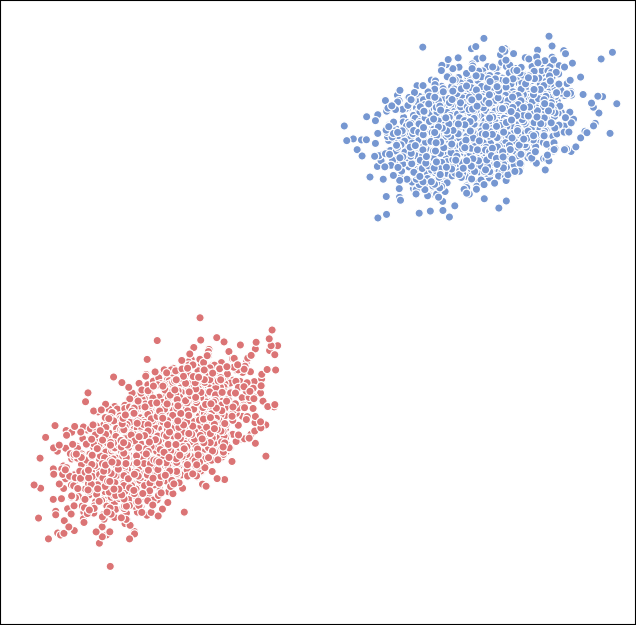
\includegraphics[width=0.3\linewidth]{Dissertation/images/ch2/metrics/ideal.png}}
        \hfill
        \subcaptionbox{второй класс вложен в первый\label{fig:metrics_cases_one_inside}}{%
            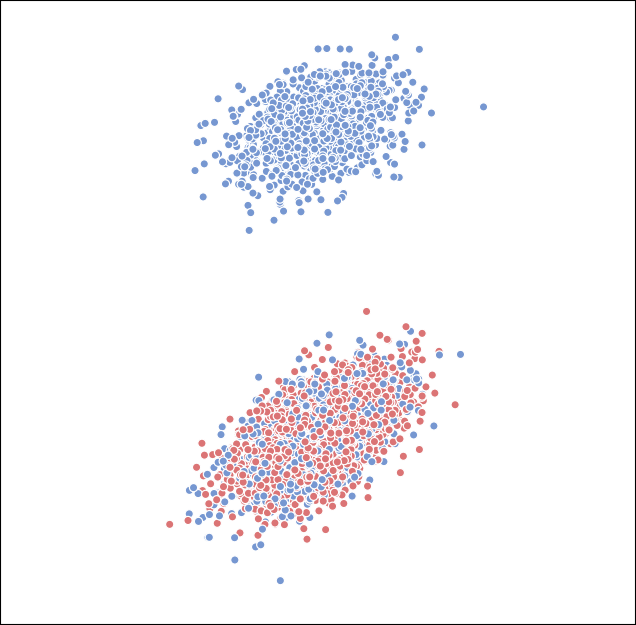
\includegraphics[width=0.3\linewidth]{Dissertation/images/ch2/metrics/second_inside.png}}
        \hfill
        \subcaptionbox{совпадающие классы\label{fig:metrics_cases_identical}}{%
            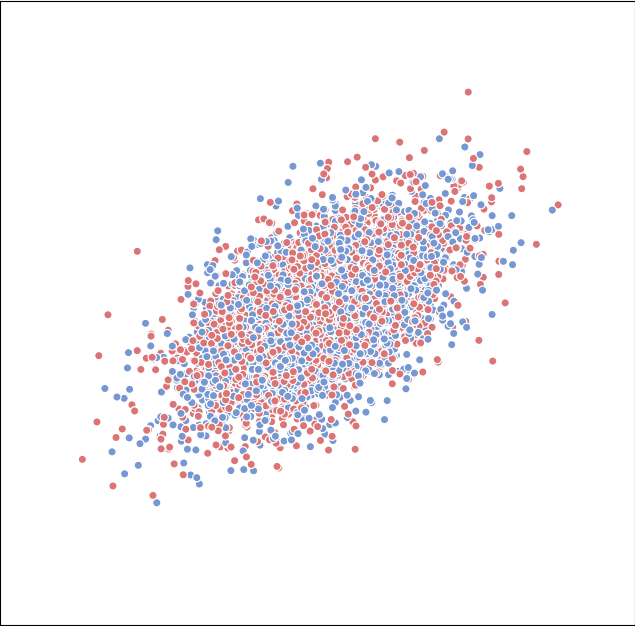
\includegraphics[width=0.3\linewidth]{Dissertation/images/ch2/metrics/identical.png}}
        \hfill
    }
    \caption{Модельные ситуации для анализа метрик}
    \label{fig:metrics_cases}
\end{figure}

Таким образом, видно, что предложенные показатели позволяют различать случаи, в которых стандартные метрики дают одинаковые значения, но интерпретация существенно различается.

\subsection{Обобщение на многоклассовый случай}

Для системы из \(C > 2\) унарных классификаторов аналогичные метрики могут быть вычислены попарно для каждой пары классификаторов, что позволяет получить полную картину взаимодействия классов. В то же время для оценки качества отдельных классификаторов достаточно использовать показатели мощности, а для анализа пересечений и эффективности -- соответствующие обобщённые гармонические средние по всем парам. Такой подход обеспечивает более информативную и детализированную оценку по сравнению с традиционными многоклассовыми метриками и учитывает особенности работы унарной схемы: независимость классификаторов, возможность отказа и линейную масштабируемость по числу классов.
